\subsection{$\alpha$ rozpad}
	Rozpad $\alpha$, například rozpad radia na radon\footnote{
		Použitá notace je ${}^{A}_{Z}\mathrm{X}$, kde $A=N+Z$ je celkový počet nukeonů nuklidu $\mathrm{X}$, $N$ je počet neutronů a $Z$ počet protonů = náboj jádra.
	}
	\begin{equation}
		{}^{224}_{\ 88}\mathrm{Ra}\stackrel{T_{1/2}=3.6\text{ dní}}{\longrightarrow}{}^{220}_{\ 86}\mathrm{Rn}+{}^{4}_{2}\mathrm{He}
	\end{equation}
	lze popsat modelem založeným na WKB aproximaci, který i přes svoji jednoduchost dává předpovědi, které kvalitativně souhlasí s experimentem.
	Představme si, že $\alpha$ částice vázaná v jádře tuneluje Coulombickou bariérou.
	Celý problém popíšeme jednorozměrným potenciálem (viz obrázek~\ref{fig:AlphaDecay})
	\begin{equation}
		V(x)=
			\begin{cases}
				-V_{0} & \text{pro }\abs{x}<a \\
				\frac{Z_{\alpha}Z\gamma}{x} & \text{pro }\abs{x}>a,
			\end{cases}
		\label{eq:AlphaDecayPotential}
	\end{equation}
	kde $Z$ je protonové číslo jádra, $Z_{\alpha}=2$ protonové číslo $\alpha$ částice, $V_{0}$ je kladný parametr,
	$\gamma=\alpha\hbar c=\frac{e^{2}}{4\pi\epsilon_{0}}$ a $\alpha$ je konstanta jemné struktury.

	\begin{figure}[!htbp]
		\centering
		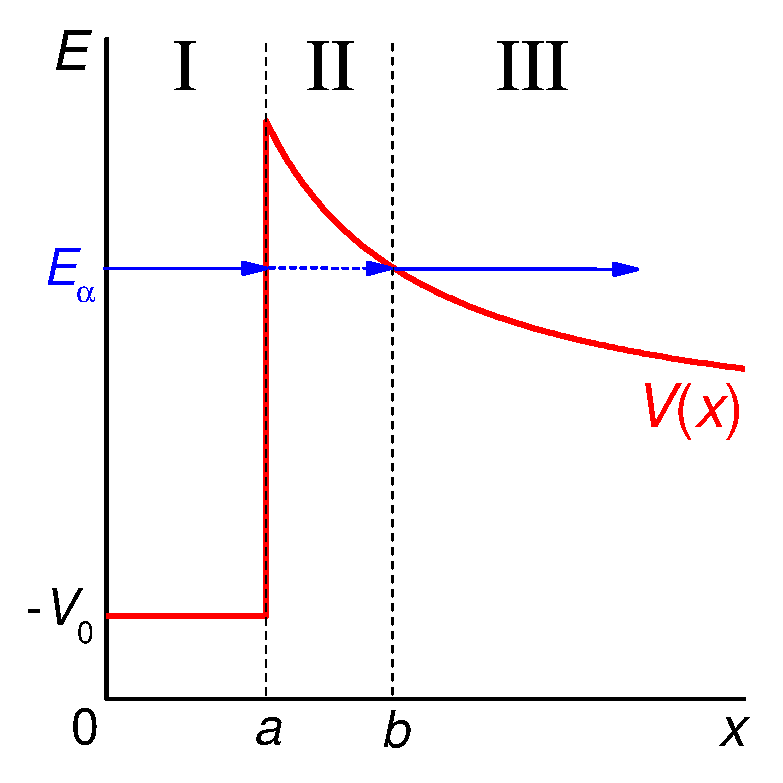
\epsfig{file=decay.eps,width=0.45\linewidth,keepaspectratio}
		\caption{
			Tunelování $\alpha$ částice o energii $E_{\alpha}$ z jádra přes Coulombickou bariéru.
		}
		\label{fig:AlphaDecay}
	\end{figure}	

	\begin{enumerate}
		\item 
			Ve WKB přiblížení odvoďte tzv. \emph{Gammovův koeficient průchodu}\index{koeficient průchodu!Gammovův}
			\begin{equation}
				\label{eq:Gammov}
				\important{
					T=\exp\left[-{\frac{2}{\hbar}}\int_{a}^{b}\abs{p(x)}\d x\right]
				},
			\end{equation}
			kde $\abs{p(x)}$ je absolutní hodnota \uv{hybnosti} částice v klasicky nedostupné oblasti vymezené body $a$, $b$, které ohraničují bariéru.
		
		\item				
			Nalezněte $T$ pro uvažovaný model $\alpha$ rozpadu.
		
		\item
			Střední dobu života lze aproximovat vztahem $\tau=\frac{1}{P_{\alpha}RT}$, kde $P_{\alpha}$ je pravděpodobnost,
			že se v jádře vydělí $\alpha$ částice (budeme předpokládat, že tato pravděpodobnost bude
			pro uvažovaná jádra $\approx1$) a $R$ je počet \uv{nárazů} $\alpha$ částice na bariéru za sekundu.
			Odhadněte $R$ a spočítejte $\tau$ a poločas rozpadu $T_{1/2}$.
		
		Pro poloměr atomu použijte přibližný vztah $a=a_{0}\sqrt[3]{A}$, kde $A$ je atomové číslo a $a_{0}\doteq1,\!2$ fm.
		
		\item
			Porovnejte číselně s hodnotami tří izotopů s poločasy rozpadu
			
			\begin{center}
				\begin{tabular}{|c|c|c|}
					\hline
					izotop & E (MeV) & $T_{1/2}$\\
					\hline
					\hline
					$^{144}_{\ 60}{\text{Nd}}$ & $1.8$ & $2\cdot10^{15}$ let\\
					\hline
					$^{224}_{\ 88}{\text{Ra}}$ & $5.7$ & $3.6$ dne\\
					\hline
					$^{212}_{\ 84}{\text{Po}}$ & $8.8$ & $0.3\,\mu$s\\
					\hline
				\end{tabular}
			\end{center}
		
		\item
			Určete de Broglieovy vlnové délky $\alpha$ částic v jádrech z tabulky a porovnejte je s rozměry jádra.
			Je WKB aproximace oprávněná?
		
	\end{enumerate}
	
\begin{solution}
	\begin{enumerate}
	\item
		Proces tunelování se rozdělí na tři oblasti:
		\begin{itemize}
		\item
			Oblast I: $x<a$, $E>V(x)$, vnitřek jádra.
		\item
			Oblast II: $a<x<b$, $E<V(x)$, Coulombická bariéra.
		\item
			Oblast III: $b<x$, $E>V(x)$, oblast vně jádra.
		\end{itemize}
		
		V oblasti III vně jádra je nenulová jen ta část vlnové funkce, která odpovídá prošlé částici vzdalující se od atomu,
		\begin{align}
			\psi_{\mathrm{III}}(x)
				&=\frac{C}{\sqrt{\abs{p(x)}}}\e^{\frac{\im}{\hbar}\int_{b}^{x}\abs{p(x')}\d x'+\im\frac{\pi}{4}}
				 =\lambda\e^{\im\left(I_{b}^{x}+\frac{\pi}{4}\right)}\nonumber\\
				&=\lambda\cos{\left[I_{b}^{x}+\frac{\pi}{4}\right]}+\im\lambda\sin{\left[I_{b}^{x}+\frac{\pi}{4}\right]},
		\end{align}
		kde je využito značení~\eqref{eq:WKBNotation}. 
		Do výrazu byla navíc přidána fáze $\pi/4$, což usnadní následné navazování vlnové funkce.
		Vlnová funkce v oblasti II se určí pomocí navazovacích vztahů~\eqref{eq:WKBConnectionDown1}---\eqref{eq:WKBConnectionDown2},
		\begin{equation}
			\psi_{\mathrm{II}}(x)=\lambda\e^{I_{x}^{b}}+\frac{\im}{2}\lambda\e^{-I_{x}^{b}}.
		\end{equation}
		
		Pomocí rozepsání integrálu
		\begin{align}
			\int_{x}^{b}&=\int_{a}^{b}-\int_{a}^{x} && \Longleftrightarrow & I_{x}^{b}&=I_{a}^{b}-I_{a}^{x}
		\end{align}
		a zkráceného označení
		\begin{equation}
			F\equiv\e^{-I_{a}^{b}}=\e^{-\frac{1}{\hbar}\int_{a}^{b}\abs{p(x)}\d x},
		\end{equation}
		vlnová funkce přejde do tvaru
		\begin{equation}
			\psi_{\mathrm{II}}(x)=\frac{\lambda}{F}\e^{-I_{a}^{x}}+\frac{\im}{2}\lambda F\e^{I_{a}^{x}}.
		\end{equation}
		Do oblasti I se následně naváže pomocí sešívacích podmínek~\eqref{eq:WKBConnectionUp1}---\eqref{eq:WKBConnectionUp2}:
		\begin{align}
			\psi_{\mathrm{I}}(x)
				&=\frac{2\lambda}{F}\sin\left[I_{a}^{x}+\frac{\pi}{4}\right]+\frac{\im}{2}\lambda F\cos\left[I_{a}^{x}+\frac{\pi}{4}\right]\nonumber\\										
				&=\underbrace{-C\left(\frac{1}{F}-\frac{F}{4}\right)\e^{\im\frac{\pi}{4}}}_{A}\frac{1}{\sqrt{\abs{p(x)}}}\e^{\im I_{x}^{a}}
					+\underbrace{\im C\left(\frac{1}{F}+\frac{F}{4}\right)\e^{-\im\frac{\pi}{4}}}_{B}\frac{1}{\sqrt{\abs{p(x)}}}\e^{-\im I_{x}^{a}}.						
		\end{align}
		Transmisní koeficient tedy vychází
		\begin{equation}
			T=\abs{\frac{C}{A}}^{2}=\frac{1}{\left(\frac{1}{F}-\frac{F}{4}\right)^{2}}\approx F^{2}\,,
		\end{equation}
		přičemž poslední rovnost platí za předpokladu $F\ll1$, což musí být splněno, aby bylo vůbec možné pro tento typ úlohy WKB aproximaci použít.
		Dosazení za $F$ dá hledaný Gammovův faktor~\eqref{eq:Gammov}.
		
	\item
		Do právě odvozeného Gammova vztahu pro pravděpodobnost průniku bariérou dosadíme potenciál~\eqref{eq:AlphaDecayPotential}.
		Klasická hybnost $\alpha$ částice o energii $E_{\alpha}$ v oblasti Coulombické části potenciálu je
		\begin{equation}
			p(x)=\sqrt{2M\left(E_{\alpha}-\frac{Z_{\alpha}Z\gamma}{x}\right)}.
		\end{equation}
		První bod obratu $a$ odpovídá poloměru jádra, druhý bod obratu se vypočítá z rovnice
		\begin{align}
			\label{eq:AlphaDecayTurningPoint}
			V(x)&=E_{\alpha} && \Longrightarrow & b&=\frac{Z_{\alpha}Z\gamma}{E_{\alpha}}\,,
		\end{align}
		takže
		\begin{align}
			I_{a}^{b}=\frac{1}{\hbar}\int_{a}^{b}\abs{p(x)}\d x
				&=\frac{\sqrt{2ME_{\alpha}}}{\hbar}\int_{a}^{b}\sqrt{\frac{Z_{\alpha}Z\gamma}{E_{\alpha}x}-1}\,\d x=\equationcomment{u=\frac{x}{b} \\ \d x=b\,\d u}\nonumber\\
				&=\underbrace{\frac{Z_{\alpha}Z\gamma}{\hbar}\sqrt{\frac{2M}{E_{\alpha}}}}_{\kappa}\int_{x=a}^{x=b}\sqrt{\frac{1}{u}-1}\,\d u=\equationcomment{u=y^{2} \\ \d u=2y\d y}\nonumber\\				
				&=2\kappa\int_{x=a}^{x=b}\sqrt{1-y^{2}}\,\d y,
		\end{align}
		což je tentýž integrál jako u WKB řešení harmonického oscilátoru~\eqref{eq:intsqrt} s primitivní funkcí
		\begin{align}
			I_{a}^{b}
				&=\kappa\left[y\sqrt{1-y^{2}}+\arcsin{y}\right]_{x=a}^{y=b}\nonumber\\
				&=\kappa\left[\sqrt{u}\sqrt{1-u}+\arcsin{\sqrt{u}}\right]_{u=\frac{a}{b}}^{1}=\nonumber\\
				&=\kappa\left[\arccos{\sqrt{\frac{a}{b}}}-\sqrt{\frac{a}{b}\left(1-\frac{a}{b}\right)}\right].
		\end{align}
		Pravděpodobnost průniku tedy vychází
		\begin{equation}
			T=\exp{\left\{\frac{2Z_{\alpha}Z\gamma}{\hbar}\sqrt{\frac{2M}{E_{\alpha}}}\left[\arccos{\sqrt{\frac{a}{b}}}-\sqrt{\frac{a}{b}\left(1-\frac{a}{b}\right)}\right]\right\}}
		\end{equation}
		kde $b$ je dáno vzorcem~\eqref{eq:AlphaDecayTurningPoint} a $a$ je poloměr jádra spočtený pomocí vztahu uvedeného v zadání příkladu.
		
	\item
		Počet \uv{nárazů} $\alpha$ částice na bariéru se odhadne jako
		\begin{equation}
			R=\frac{v_{\alpha}}{2a},
		\end{equation}
		kde $v_{\alpha}$ je rychlost $\alpha$ částice v jádře.
		Tu určíme z kinetické energie.
		Stačí počítat pomocí nerelativistických vztahů, protože rychlost vylétávajících $\alpha$ částic je malá ve srovnání s rychlostí světla, jak se lze přesvědčit z tabulky níže:
		\begin{equation}
			E_{\alpha}=v_{\alpha}^{2}/2M,
		\end{equation}
		přičemž energie je dána jako rozdíl klidové hmotnosti $M_{{}^{A}_{Z}X}$ jádra vstupujícího do reakce a klidové hmotnosti produktů (jádro $M_{{}^{A-4}_{Z-2}Y}$ + jádro helia $M_{{}^{4}_{2}\mathrm{He}}$)
		\begin{equation}
			E_{\alpha}=\frac{1}{c^{2}}\left(M_{{}^{A}_{Z}X}-M_{{}^{A-4}_{Z-2}Y}-M_{{}^{4}_{2}\mathrm{He}}\right)\,.
		\end{equation}
		Rychlost tedy vychází
		\begin{equation}
			v_{\alpha}=\sqrt{\frac{2\left(E_{\alpha}+V_{0}\right)}{M}}
		\end{equation}
		a z ní střední doba života
		\begin{equation}
			\tau=\frac{2a}{T}\sqrt{\frac{M}{2\left(E_{\alpha}+V_{0}\right)}}.
		\end{equation}
		Poločas rozpadu je $T_{1/2}=\tau\ln2$.

	\item
		Výsledky pro zadané izotopy jsou v následující tabulce:
		\begin{center}
			\begin{tabular}{|c|c|c|c|c|c|c|c|c|c|}
				\hline
				izotop & $\begin{array}{c}E_{\alpha} \\ \text{(MeV)}\end{array}$ & $\begin{array}{c}a \\ \text{(fm)}\end{array}$ & $\begin{array}{c}b \\ \text{(fm)}\end{array}$ 
				& $\frac{v_{\alpha}}{c}$ & $I_{a}^{b}$ & T & $\begin{array}{c}T_{1/2} \\ (s)\end{array}$ & $T_{1/2}$ \\
				\hline
				\hline
				$^{144}_{\ 60}{\text{Nd}}$ & $1.8$ & $6.3$ & $96$ & $0.17$ & $120$ & $7.2\cdot10^{-53}$ & $2.4\cdot10^{30}$ & $7.6\cdot10^{22}$ let \\
				\hline
				$^{224}_{\ 88}{\text{Ra}}$ & $5.7$ & $7.3$ & $45$ & $0.17$ & $73$ & $2.3\cdot10^{-32}$ & $8.5\cdot10^{9}$ & $98000$ dní \\
				\hline
				$^{212}_{\ 84}{\text{Po}}$ & $8.8$ & $7.2$ & $28$ & $0.18$ & $43$ & $3.1\cdot10^{-19}$ & $5.9\cdot10^{-4}$ & $590$ $\mu$s\\
				\hline
			\end{tabular}
		\end{center}
		Tento velmi zjednodušený výpočet tedy dává o několik řádů delší poločasy rozpadu, než jsou naměřené hodnoty ze zadání příkladu.
		Mnohem lepší shody se dosáhne, pokud se uvažuje $a_{0}=1.6$ fm, což v sobě může zahrnout difuzivitu jaderného povrchu.
		
	\item
		De Broglieovy vlnové délky $\alpha$ částic jsou
		\begin{equation}
			\lambda_{\alpha}=\frac{p_{\alpha}}{\hbar}=\frac{Mv_{\alpha}}{\hbar}\,.
		\end{equation}
		Číselně
		\begin{center}
			\begin{tabular}{|c|c|}
				\hline
				izotop & $\lambda_{\alpha}$ (fm) \\
				\hline
				\hline
				$^{144}_{\ 60}{\text{Nd}}$ & $0.32$ \\
				\hline
				$^{224}_{\ 88}{\text{Ra}}$ & $0.31$ \\
				\hline
				$^{212}_{\ 84}{\text{Po}}$ & $0.30$ \\
				\hline
			\end{tabular}
		\end{center}
		tedy asi 40 krát menší než je rozměr jádra.				
	\end{enumerate}

	\begin{note}
		Pro $a\ll b$ lze aproximovat
		\begin{equation}
			\arccos{\sqrt{\frac{a}{b}}}-\sqrt{\frac{a}{b}-\frac{a^{2}}{b^{2}}}\approx\frac{\pi}{2}-\sqrt{\frac{a}{b}}-\sqrt{\frac{a}{b}}=\frac{\pi}{2}-2\sqrt{\frac{a}{b}}\,.
		\end{equation}
		Pak
		\begin{align}
			\ln\tau
				&=\ln{\frac{2a}{v_{\alpha}}}+2I_{a}^{b}\nonumber\\
				&=\ln{\frac{2a_{0}\sqrt[3]{A}}{\sqrt{2\left(E_{\alpha}+V_{0}\right){M}}}}
					+\frac{2Z_{\alpha}Z\gamma}{\hbar}\sqrt{\frac{2M}{E_{\alpha}}}\left[\frac{\pi}{2}-2\sqrt{\frac{a_{0}}{Z_{\alpha}\gamma}}\sqrt{E_{\alpha}}A^{\frac{1}{6}}Z^{-\frac{1}{2}}\right]
		\end{align}
		a pro těžká jádra, pro která platí $A\approx 2Z$, dostaneme
		\begin{align}
			\ln\tau&=\frac{1}{3}\ln{Z}+\frac{1}{3}\ln{2}+\ln{\frac{2a_{0}}{\sqrt{\frac{2\left(E_{\alpha}-V_{0}\right)}{M}}}}+\frac{2Z_{\alpha}\gamma\sqrt{2M}}{\hbar}\frac{\pi}{2}\frac{Z}{\sqrt{E}}
				-4\frac{\sqrt{2Z_{\alpha}\gamma a_{0}M}}{\hbar}\sqrt[6]{2}Z^{\frac{2}{3}}
		\end{align}
		To je v souladu s experimentálně pozorovanou závislostí
		\begin{equation}
			(\ln{\tau})_{\mathrm{exp}}=C_{1}\left(\frac{Z}{\sqrt{E_{\alpha}}}-Z^{\frac{2}{3}}\right)-C_{2}\,.
		\end{equation}
	\end{note}
\end{solution}
